\documentclass[12pt,reqno,final]{amsart}
\usepackage[round,numbers,sort&compress]{natbib}
\usepackage{graphicx}
\usepackage{times}
\usepackage{rotating}
\usepackage{subfig}

\title[DEB fitting notes]{Fitting Dynamic Energy Budget Models: Notes}

\setlength{\textwidth}{6.25in}
\setlength{\textheight}{8.75in}
\setlength{\evensidemargin}{0in}
\setlength{\oddsidemargin}{0in}
\setlength{\topmargin}{-.35in}
\setlength{\parskip}{.1in}
\setlength{\parindent}{0.0in}

\theoremstyle{plain}
\newtheorem{thm}{Theorem}
\newtheorem{corol}[thm]{Corollary}
\newtheorem{prop}[thm]{Proposition}
\newtheorem{lemma}[thm]{Lemma}
\newtheorem{defn}[thm]{Definition}
\newtheorem{hyp}[thm]{Hypothesis}
\newtheorem{example}[thm]{Example}
\newtheorem{conj}[thm]{Conjecture}
\newtheorem{algorithm}[thm]{Algorithm}
\newtheorem{remark}{Remark}
\renewcommand\thethm{\arabic{thm}}
\renewcommand{\theremark}{}

\numberwithin{equation}{part}
\renewcommand\theequation{\arabic{equation}}
\renewcommand\thesection{\arabic{section}}
\renewcommand\thesubsection{\thesection.\arabic{subsection}}
\renewcommand\thefigure{\arabic{figure}}
\renewcommand\thetable{\arabic{table}}
\renewcommand\thefootnote{\arabic{footnote}}

\usepackage{Sweave}
\begin{document}

\maketitle

I have fit all of Adriana's data and determined the best fitting
parameter set for each animal of each genotype. For each animal of
each genotype, I have also recorded the observed age at death, the
observed mean daily egg rate, and Adriana's fitted von Bertalanffy
$L_{inf}$ value. Additionally, I have used the best fit parameter
values to compute growth and reproduction trajectories, and then
calculated a predicted mean daily egg rate and $L_{max}$ (maximum
predicted length, distinct from von Bertalanffy $L_{inf}$). I also
used NLS to fit von Bertalanffy growth curves to each trajectory, as
Adriana did, and recorded the best fit $k$ and $L_{inf}$ parameters. I
then went back and refit all the individual trajectories, fitting only
$L_{inf}$, with $k$ held at the mean $k$ for all of the previous
fittings. I then calculated $\kappa_1 = L_{inf}\bar{k}$ so I
could compare it against Adriana's $\kappa_1$, where she had estimated
$\bar{k} = 0.161$.

The first thing I want to look at is the correlation between Adriana's
$\kappa_1$ and the predicted $\kappa_1$, and between the observed and
predicted mean daily egg rates. I also show the correlation between
life history characteristics (growth rate $\kappa_1$, mean daily egg
rate, and age at death) as computed by Adriana, and using the
predicted trajectories. Adriana's life history characteristics are shown as red
squares in each panel, and the predicted life history characteristics
are shown as black circles.

The next figure shows the partial correlation coefficients between
each life history characteristic, both observed and predicted using
the best fit parameter sets. The partial correlation is the
correlation between the residuals of two variables, after regressing
against the third, e.g., regress growth rate and egg rate against age
at death and then compute the correlation between the
residuals.

\begin{figure}
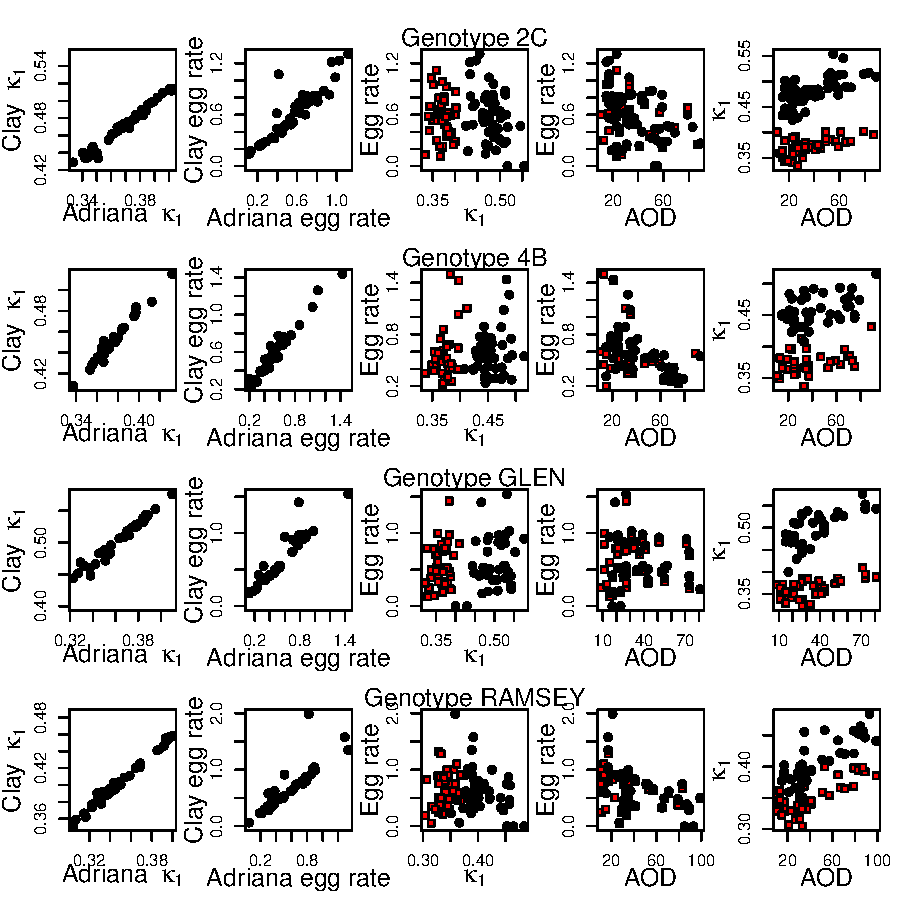
\includegraphics{Comparing_best_fit_parameters_against_Adriana_winners_and_losers-001}
\caption{Comparison of empirically-derived $\kappa_1$ growth rate
  measure and mean daily egg rate and the growth and egg rates
  calculated using the growth and reproduction trajectories from the
  best-fit parameter values.}
\end{figure}

\begin{figure}
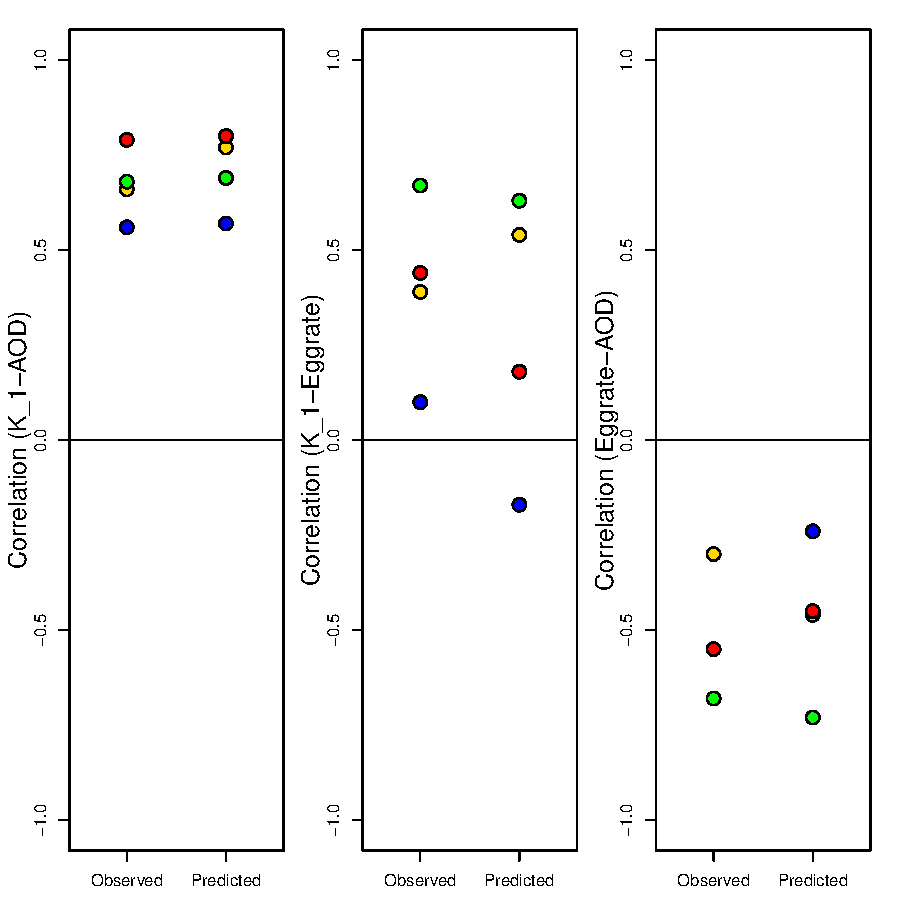
\includegraphics{Comparing_best_fit_parameters_against_Adriana_winners_and_losers-002}
\caption{Partial correlation coefficients between life history
  characteristics observed in the data and predicted using the
  trajectories generated by the best fit parameter values.}
\end{figure}

I also want to see if the empirically-observed high fliers have
parameter values that cluster together. To show this, I am going to
plot the distributions of the estimated parameters, and I will color
those parameter estimates that came from individuals with mean daily
egg rates in the top 25\% red (Figs. 3-6).  I also show these distributions with
individuals with $L_{inf}$ values in the top 25\% colored red (Figs. 7-10).

\begin{figure}
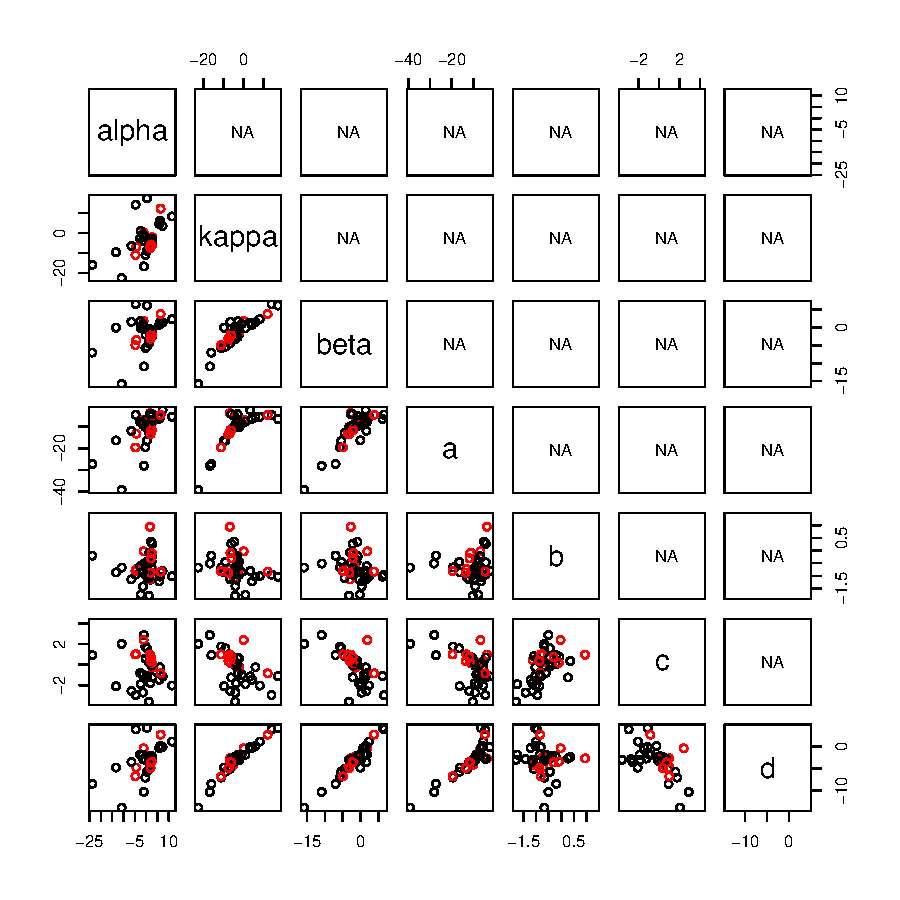
\includegraphics{Comparing_best_fit_parameters_against_Adriana_winners_and_losers-003}
\caption{For genotype 2C, the correlations amongst the best fit
  parameter values. The top 25\% of reproducers are shown in red.}
\end{figure}

\begin{figure}
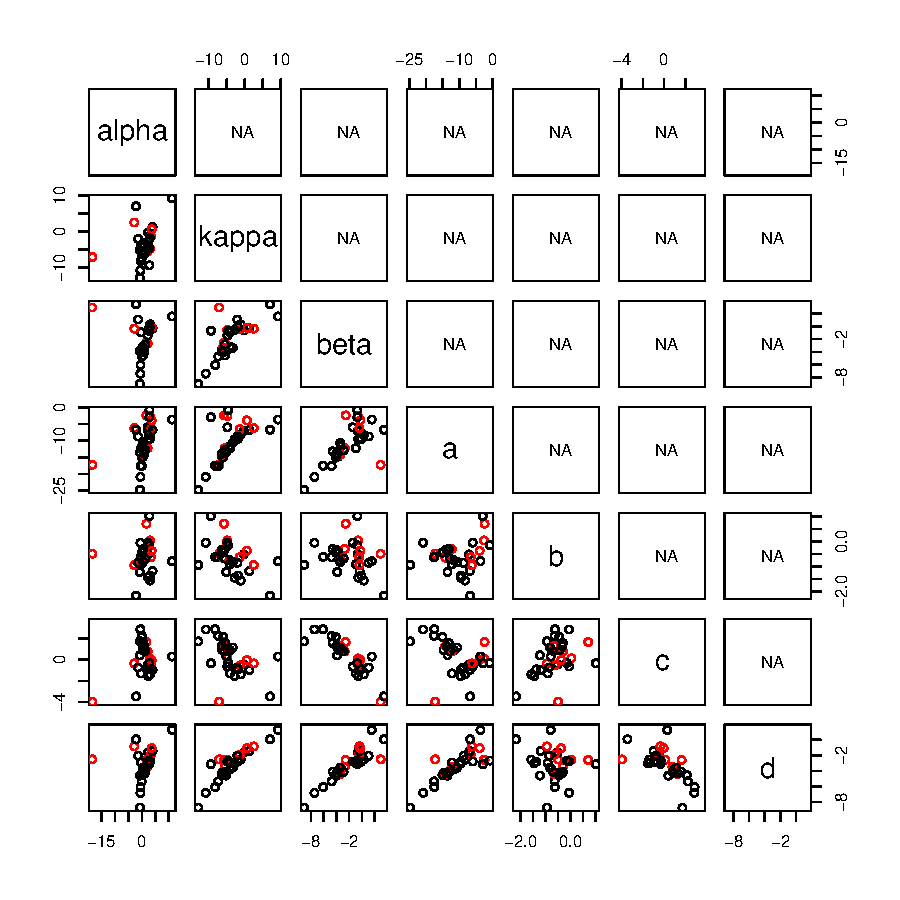
\includegraphics{Comparing_best_fit_parameters_against_Adriana_winners_and_losers-004}
\caption{For genotype 4B, the correlations amongst the best fit
  parameter values. The top 25\% of reproducers are shown in red.}
\end{figure}

\begin{figure}
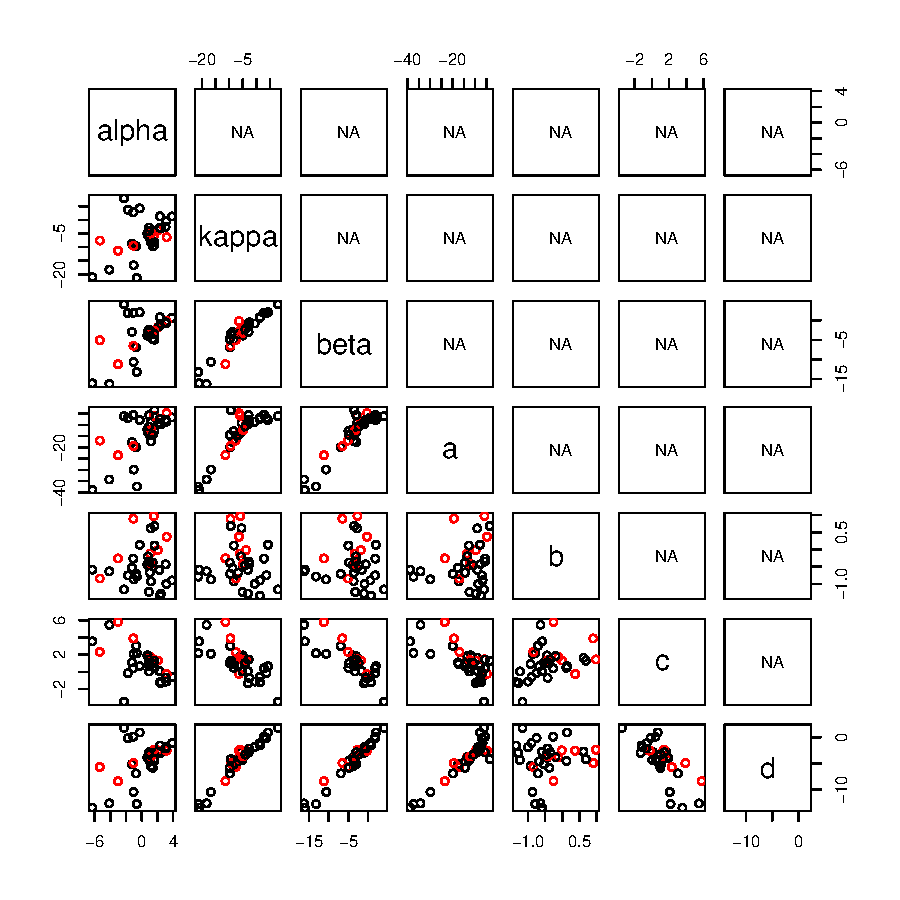
\includegraphics{Comparing_best_fit_parameters_against_Adriana_winners_and_losers-005}
\caption{For genotype GLEN, the correlations amongst the best fit
  parameter values. The top 25\% of reproducers are shown in red.}
\end{figure}

\begin{figure}
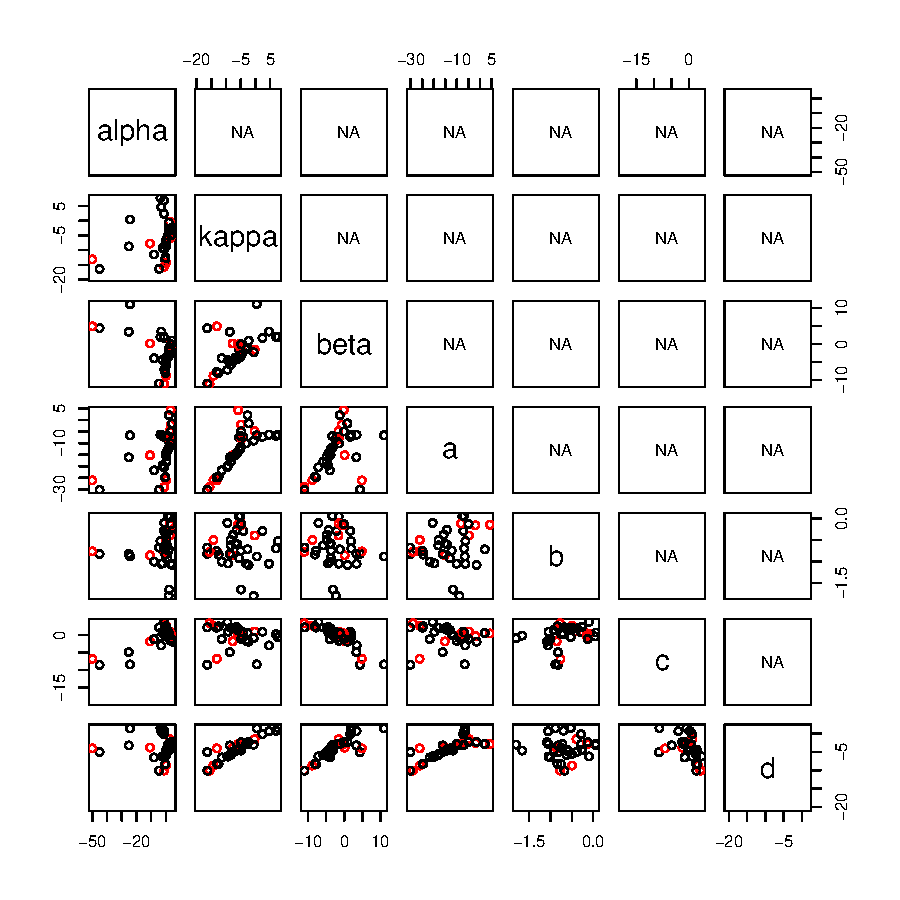
\includegraphics{Comparing_best_fit_parameters_against_Adriana_winners_and_losers-006}
\caption{For genotype RAMSEY, the correlations amongst the best fit
  parameter values. The top 25\% of reproducers are shown in red.}
\end{figure}

\begin{figure}
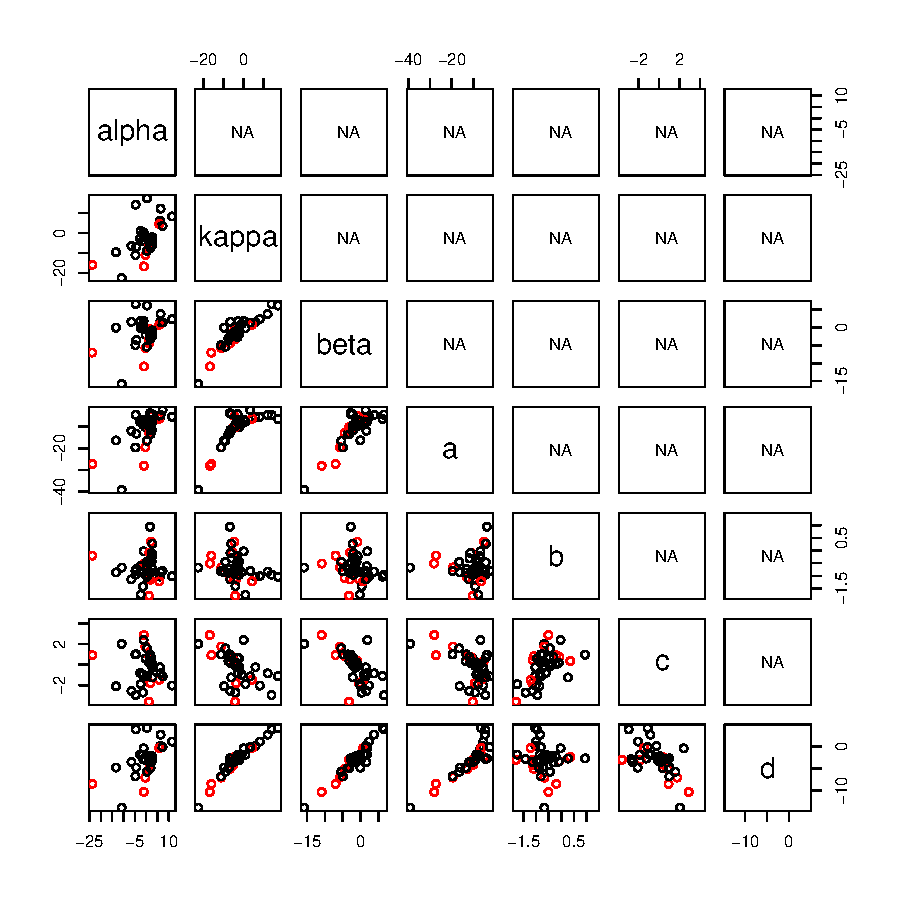
\includegraphics{Comparing_best_fit_parameters_against_Adriana_winners_and_losers-007}
\caption{For genotype 2C, the correlations amongst the best fit
  parameter values. The top 25\% of growers are shown in red.}
\end{figure}

\begin{figure}
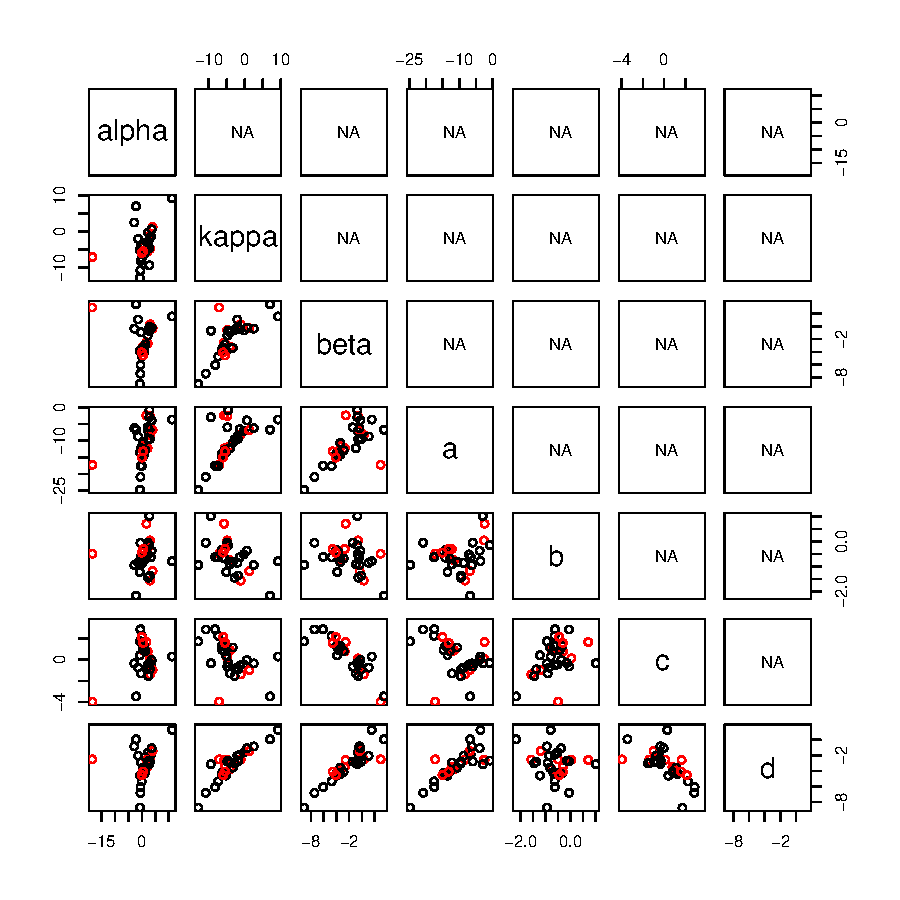
\includegraphics{Comparing_best_fit_parameters_against_Adriana_winners_and_losers-008}
\caption{For genotype 4B, the correlations amongst the best fit
  parameter values. The top 25\% of growers are shown in red.}
\end{figure}

\begin{figure}
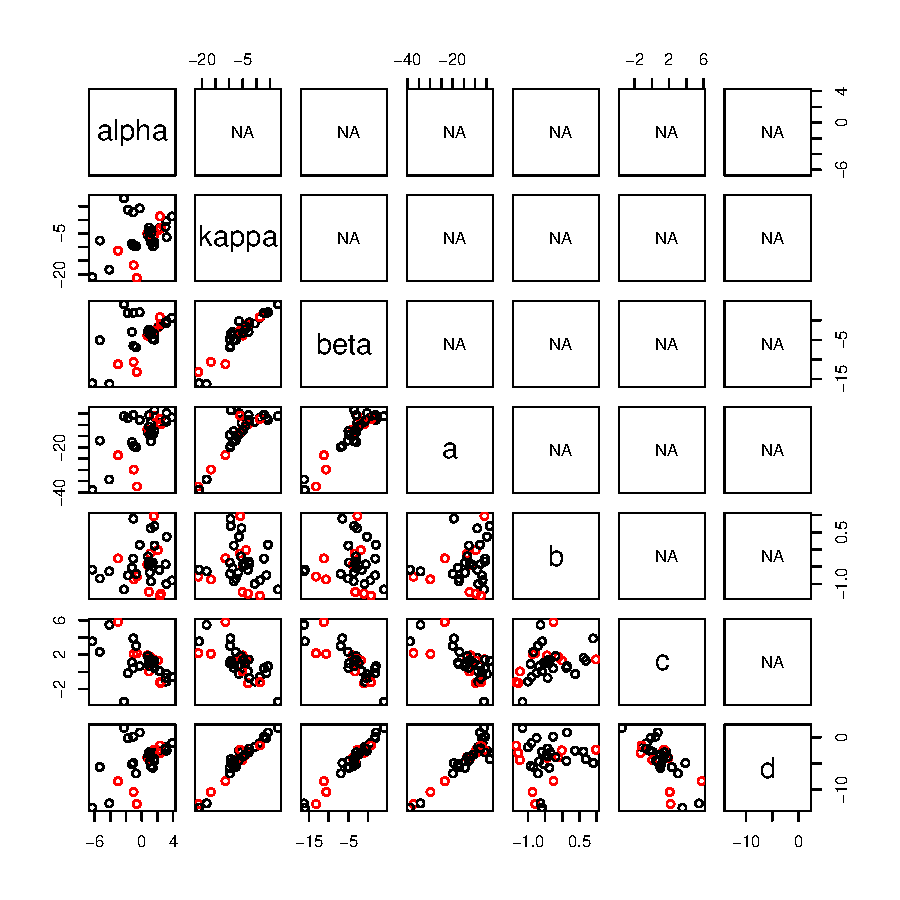
\includegraphics{Comparing_best_fit_parameters_against_Adriana_winners_and_losers-009}
\caption{For genotype GLEN, the correlations amongst the best fit
  parameter values. The top 25\% of growers are shown in red.}
\end{figure}

\begin{figure}
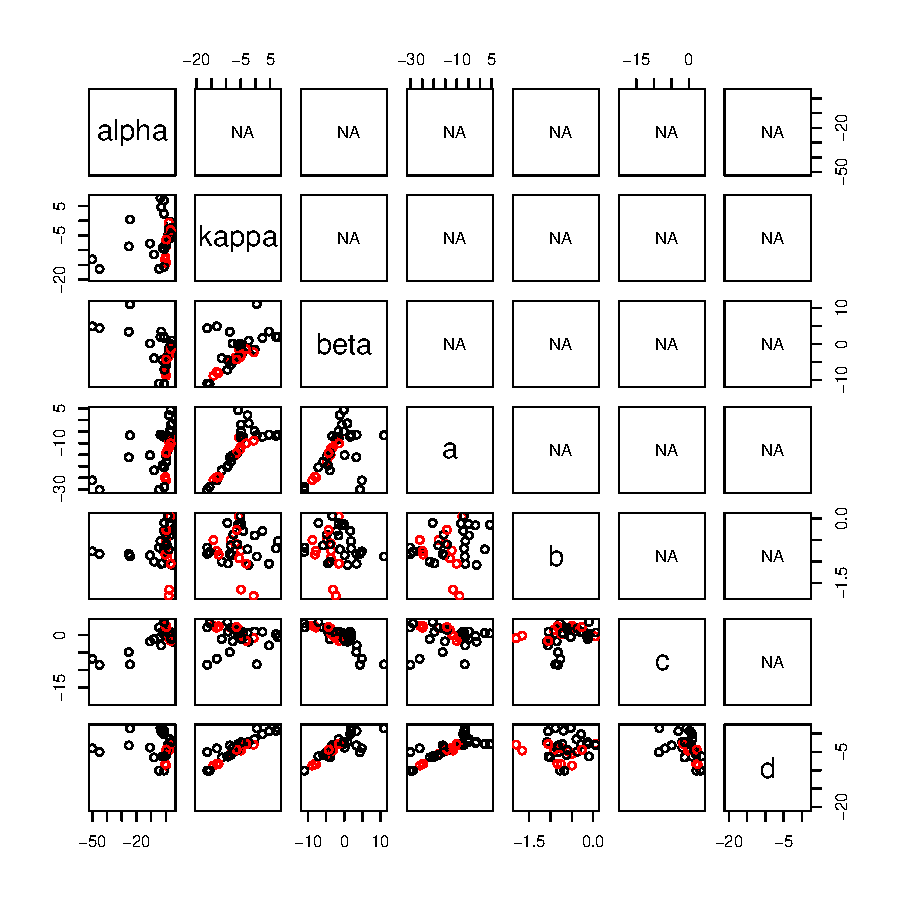
\includegraphics{Comparing_best_fit_parameters_against_Adriana_winners_and_losers-010}
\caption{For genotype RAMSEY, the correlations amongst the best fit
  parameter values. The top 25\% of growers are shown in red.}
\end{figure}


\end{document}

